\documentclass[oneside]{book}
\usepackage{fullpage}
\usepackage{graphicx}

\title{\huge CS 448  Project Documentation: Confined}
\author{Alex Klen \\ ayklen \\ 20372654}

\begin{document}
\maketitle
\tableofcontents

\chapter{Introduction}
  \section{Purpose}
    The purpose of this project was to create a rendering pipeline utilizing modern OpenGL shader techniques and exhibit it with an interactive demo game.
    The focus is on implementing several graphical features in an OpenGL shader pipeline. These features must not only be compatible, but they should together build a comprehensive rendering engine.
    The demo should extensively use lights and dynamic shadows and run at an interactive frame rates.

    This project was interesting and challenging because it involves using several advanced shader techniques at the same time. I learned how to effectively use GLSL on modern hardware to achieve quality light and shadow rendering at interactive frame rates, as well as how several other popular effects are achieved in shaders.

  \section{Overview of Features}
    \begin{figure}[h!]
      \centering
      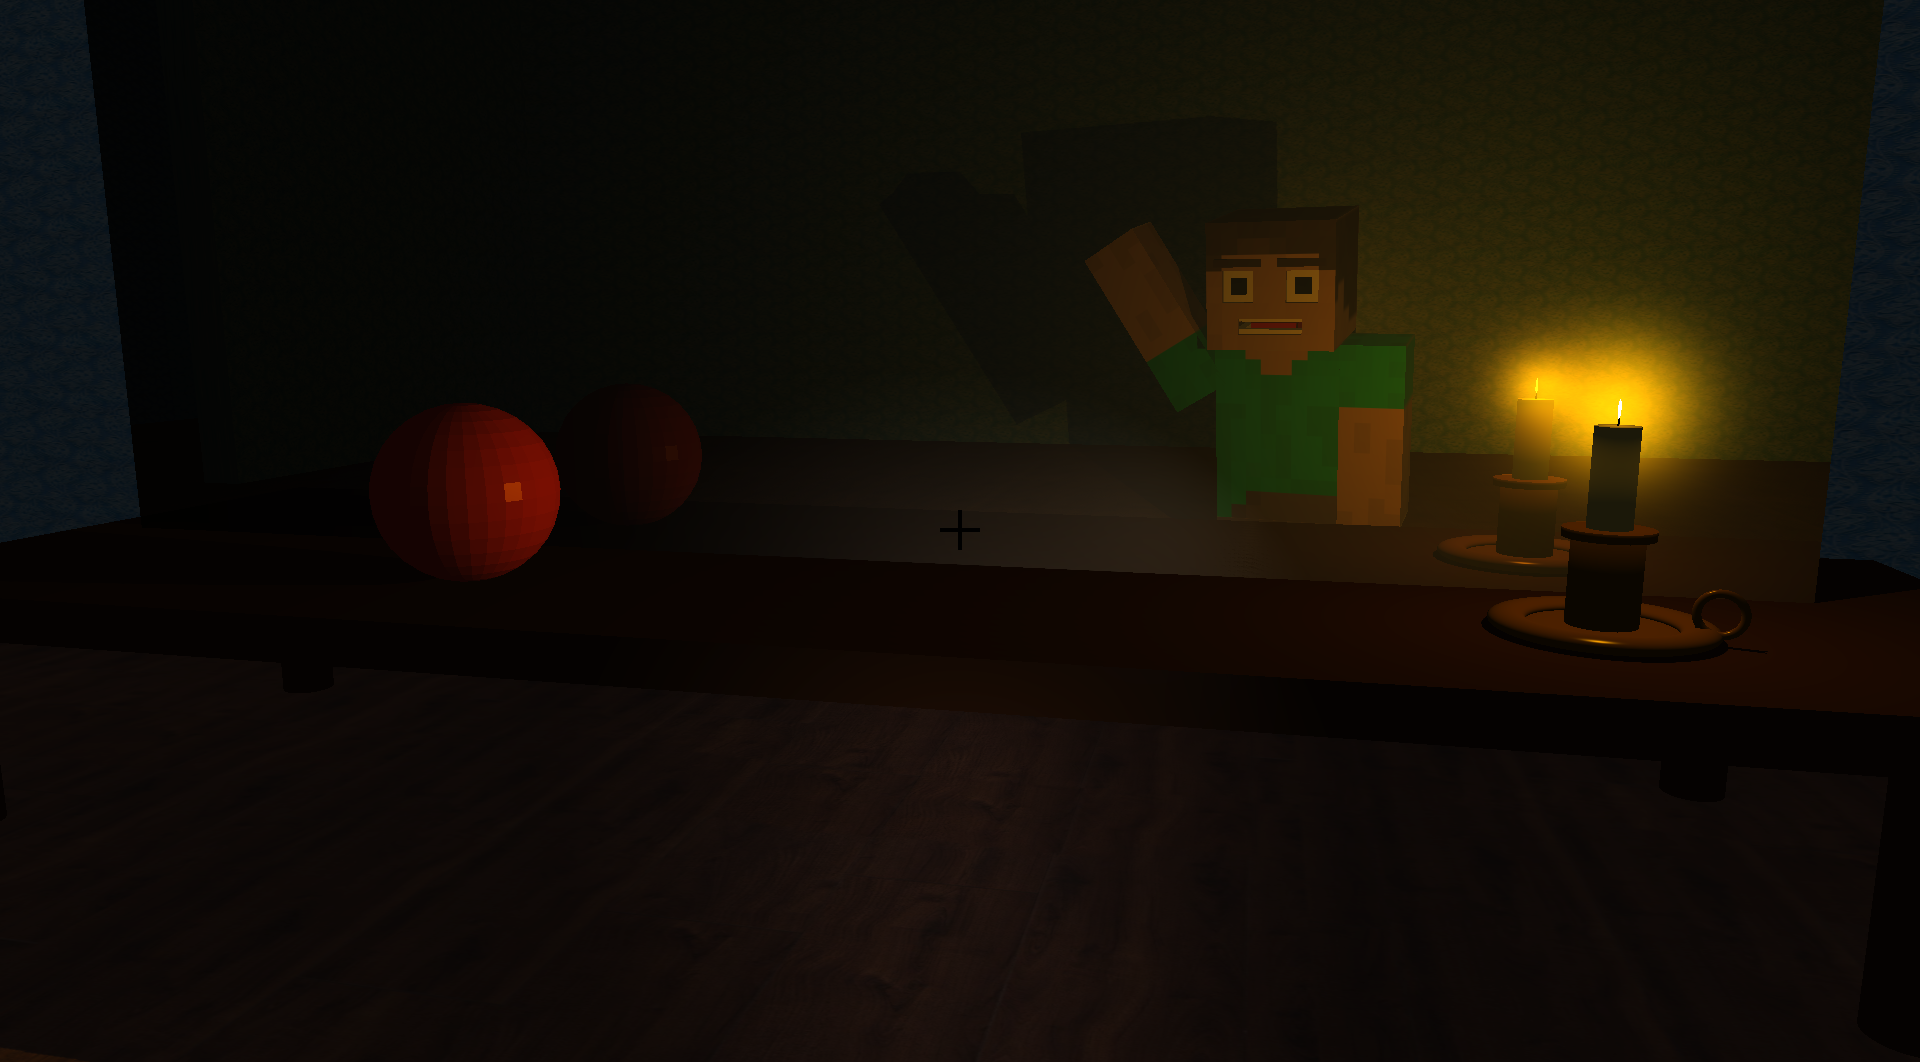
\includegraphics[width=1.0\textwidth]{../screenshot01.png}
      \caption{Screenshot of Game - Looking at self in mirror.}
      \label{screenshot01}
    \end{figure}

    Most of the rendering engine's features were objectives of the project, with a few extra features implemented as well. The features are covered in more depth and their technical aspects are discussed in Section \ref{technical-objectives}.

    The interactive demo is navigating using first-person controls, similar to first-person shooter games.
    Texture mapping and normal mapping allow high levels of detail on all the surfaces rendered with the pipeline. Textures are used as a polygon's diffuse colour if it is set. Normals for each fragment are perturbed by a tangent-space normal map to create realistic specular highlights.
    Dynamic shadow maps make a huge impact to the quality of the rendered output - it gives the player depth cues, but also makes the environment much more interesting because movements cause drastic changes in how the environment appears.
    Ambient occlusion is approximated with a technique called Screen Space Ambient Occlusion (SSAO) to improve the overall look of models. Instead of adding a constant ambient component to light partially shadowed areas and areas not in direct light, an occlusion factor is computed that approximates how much surrounding geometry covers each pixel. This causes depressions and crevices in models to be darker.

    Keyframe animation was added to allow models to dynamically change between frames. It's tedious to simply apply model transformation matrices manually - keyframes can be exported from animation software.
    Planar mirror reflection was added. It's a feature that's interesting to interact with - often to see if it works like a real-life mirror. It also allows the player to see what their character looks like in the demo and to see his animation.
    Motion blur was added as a post-processing step that smears pixels proportional to camera rotations and translations in screen space. It improves the overall look of the game when the player is moving around. It also smooths out frame changes at lower frame rates.
    Sound was added using OpenAL. Sound effects are synchronized with game interactions and when using a stereo headset they will sound like they are coming from the direction that they would be for the character in the game.

    Picking using shaders is an extra feature. Since you know which fragment is being drawn for each mesh in one of the shaders, you can use this to cheaply pick meshes.

    The rendering pipeline is implemented as a deferred rendering pipeline. This is to avoid directly shading each vertex with each light (see \ref{deferred-rendering}).

    These features can all be enabled at once to provide an immersive experience. Most of them can be disabled by pressing a number key. This can help you see their effect on rendering much better. These settings are explained in Section \ref{settings}.


\chapter{Manual}
  \section{Running the Program}
    \subsection{Hardware}
      This program requires a graphics card that supports OpenGL 3.3+.
      OpenGL 3.3+ is required for its efficient buffers, customizable rendering pipeline, and multiple render targets (required for deferred shading).
      This project was developed with an NVIDIA GTS 360M.

    \subsection{Operating System}
      This program was written to run on linux. It uses a cross-platform library for windows and I/O, so can easily be adapted to work on other platforms, but this was never attempted during development.

    \subsection{Dependencies}
      In addition to libraries typically found on linux distributions, the following libraries are dependencies of this program:
      \begin{itemize}
        \item GLEW - OpenGL extension wrangling.
        \item GLU - OpenGL utilities.
        \item glfw3 - for cross-platform windows and keyboard and mouse I/O.
        \item assimp - for importing external model files.
        \item freeimage - for image loading, saving, and conversion.
        \item openal - for sound.
        \item alut - utilities for OpenAL.
      \end{itemize}

      These should be installed on the system prior to building the program.

    \subsection{Building}
      To build the program, simply use the `make' command.
      Note that this program requires several libraries that are dynamically linked in the Makefile. They are outlined in the previous section.

    \subsection{Running}
      To run the program after building, simply run `./confined' from the command line.
      There are no command-line parameters - see Section \ref{settings} for setting configurations, which are done during runtime.
      To quit the program press `Q'.

  \section{Controls}
    \subsection{Looking Around - Mouse}
      The base controls for this program are similar to other first-person games.
      Simply move the mouse in two dimensions to change the angle you are looking in the 3D game world.
      Note that when the game is running it will capture the mouse cursor. You can either quit the program by pressing `Q' or minimize its window to regain control of the mouse cursor.

    \subsection{Movement - Keyboard}
      To navigate the 3D environment, you can use either the `WASD' keys or the arrow keys. Using the `WASD' keys is recommended if you are right-handed since it's easier to use them with your left hand while you use the mouse with your right. `W' is up, `A' is left, `S' is down, and `D' is right. Moving forwards and backwards will move you towards or away from the direction you are facing. Moving left and right will make your character strafe sideways.

      Mainly for debugging purposes, the keys `Q' and `E' make your character float up and down.

    \subsection{Special Keys}
      \begin{itemize}
        \item The `Q' key will quit the program.
        \item The `F' key will toggle your flashlight, if you have one.
        \item The space bar will trigger a short hand wave animation by your character. You'll have to either be looking in the mirror or be looking at your shadow to see it.
        \item The number keys toggle settings. See Section \ref{settings}.
      \end{itemize}

    \subsection{Taking Items and Shooting - Mouse Buttons}
      Press the right mouse button while your cross hair is over an item to pick it up. The two items you can pick up are the flashlight and the gun.

      Press the left mouse button after you have a gun to shoot it.

  \section{Playing the Demo}
    This project features a short demo to showcase the rendering engine. Following is a walkthrough of the demo.

    When the game starts (after loading for a few seconds), you will see a wall ahead of you, but everything will be quite dark. Looking to the left, you see a door with light coming through it. You can step through the door and approach a table with several items on it. The light source is a glowing candle on the right side. There is a large, flat mirror that lets you see yourself in it. Also on the table is a red sphere and a flashlight. You can pick up the flashlight by right-clicking on it. After getting the flashlight, you can press `F' to turn it on. Now that you can see farther because of the flashlight, you'll notice there is a cube with a brick texture and another door in the room. Progressing through the door leads to a room with a large window. Lighting flashes through the window periodically, with thunder sounds following. At the end of the room is a monkey figure. If you check behind the monkey figure, there is a gun on the ground that can also be picked up. After picking up the gun, you can left-click to shoot (causing a sound effect and a flash of light). Shooting toggles a light in the previous room. This light robits around the brick-textured cube. If you're feeling adventurous, you can step through a wall or float out the window to get outside. The sky is pitch black, but the grass has a nice texture and normal map you can look at.

  \section{Testing Features}
    You can test each feature of the rendering engine in this demo. Textures were mapped on the floor, walls, mirror, cube, gun, and grass. Normal maps are evident in several places. When you look at the candle from a distance, you see yellowish specular highlights on the ground. You can also point the flashlight straight down to see the floor's normal map working. After enabling the orbiting light, when it comes between you and the cube you can see the specular highlights on the brick texture line up with the texture. Shadow maps should be evident throughout the walkthrough. To test animation you can look in the mirror and press the space bar.

    SSAO must be turned on (it is off by default). You can do this by pressing the `5' key. You should also turn on blur by hitting `6' (see Section \ref{ssao}).
    Motion blur is on by default, but you need to toggle it to see the difference it makes. You can toggle motion blur with the `7' key.

  \section{Settings}\label{settings}
    The number keys toggle the following features of the rendering pipeline.
    \begin{enumerate}
      \setcounter{enumi}{-1}
      \item Diffuse Lighting
      \item Specular Lighting
      \item Shadow Maps
      \item Normal Maps
      \item Texture Maps
      \item SSAO
      \item Blur
      \item Motion Blur
      \item Mirrors
      \item Highlight Pick
    \end{enumerate}

\chapter{Technical Details}
  \section{Rendering Pipeline}
    \subsection{Deferred Rendering} \label{deferred-rendering}
      Deferred shading is a method of shading that speeds up subsequent lighting and shadow depth passes by letting them perform per-pixel lighting calculations only, instead of computing them for all geometry and all fragments \cite{ferkoreal}.

      When forward-rendering, the vertex shader will compute lighting parameters (incident, normal, colours) which will be interpolated for each fragment. Deferred shading, however, uses two passes. In the first it computes geometric parameters for each pixel and writes them to a textures for later use. Subsequent shading passes can then sample these textures and operate per-fragment only. The benefit of this is clear when you consider shadow mapping with many lights, since when forward rendering you would need to run the shadow mapping algorithm over all geometry for each light and each fragment, whereas with deferred shading you only need to do it for each fragment. Although there are many shader passes the memory bandwidth of each is quite small.


    \subsection{Confined's Rendering Pipeline}
      \begin{figure}[h!]
        \centering
        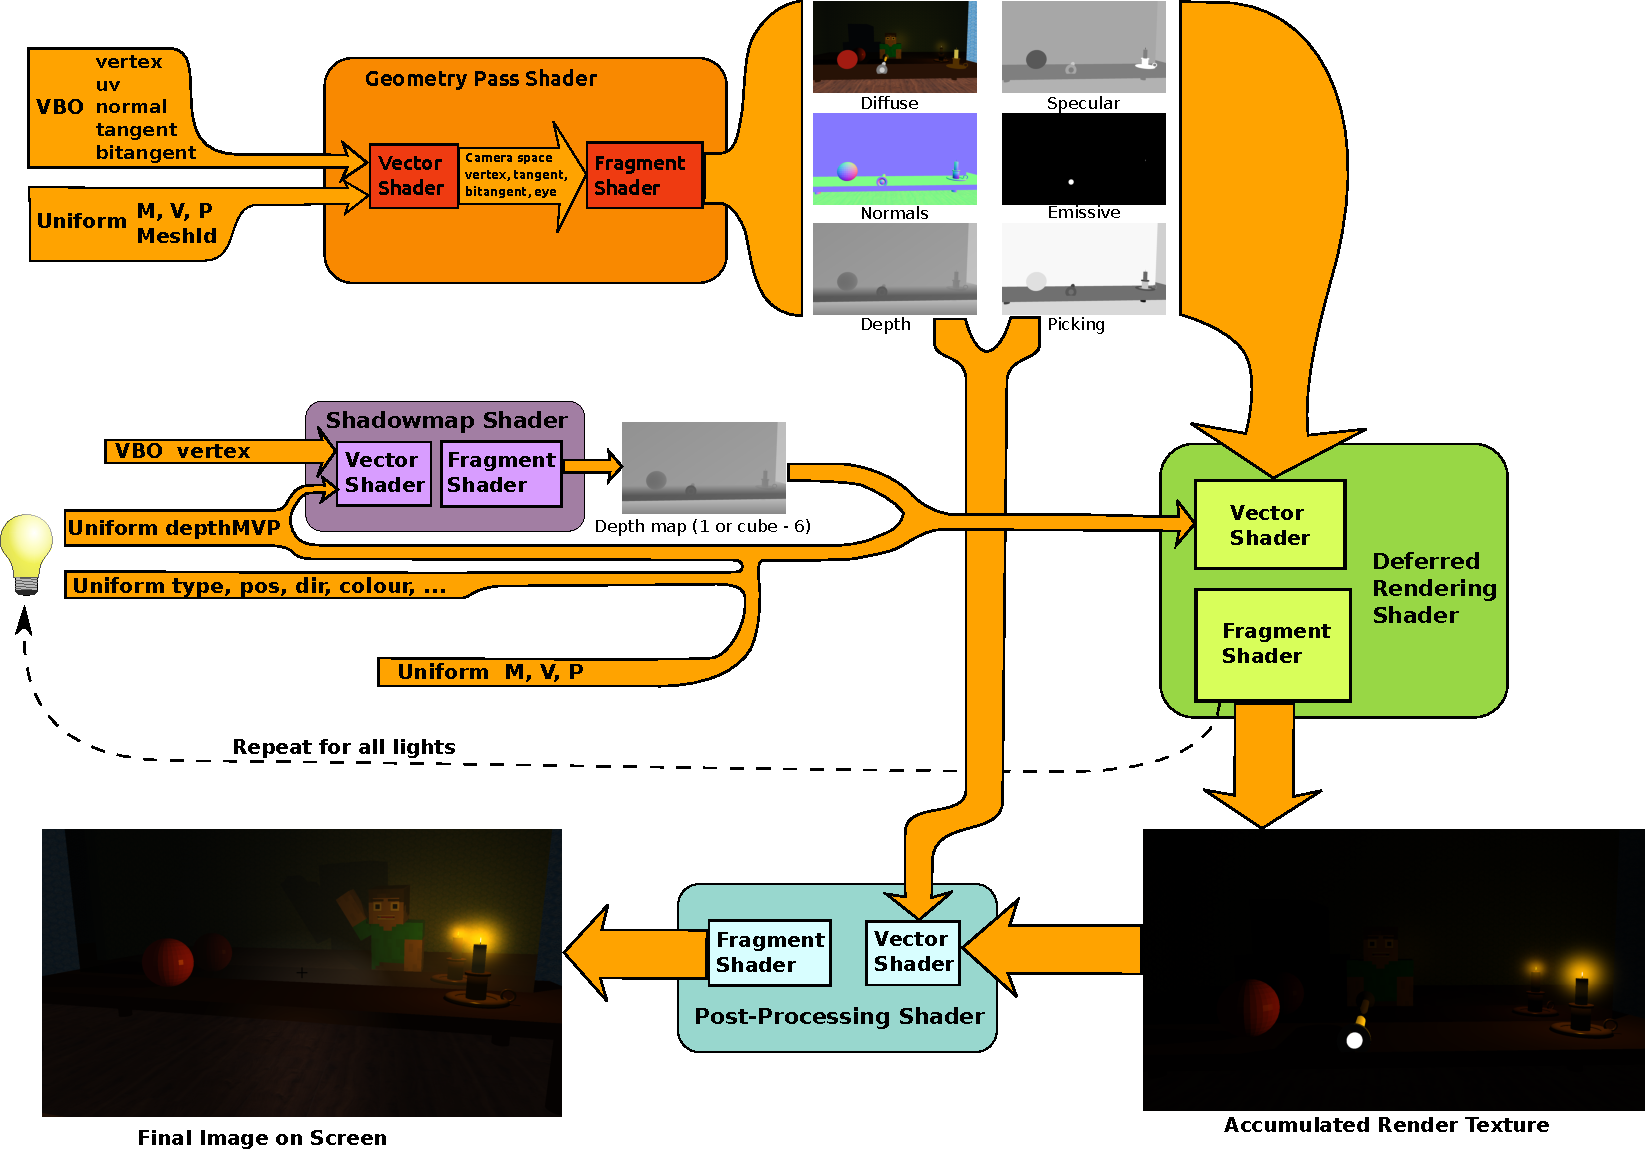
\includegraphics[width=1.0\textwidth]{rendering_pipeline}
        \caption{Rendering Pipeline}
        \label{pipeline-img}
      \end{figure}

      Figure \ref{pipeline-img} shows the overall structure and some details of the rendering pipeline.

      The Geometry Pass Shader is the first stage in deferred shading, and is responsible for taking scene data and creating 6 output render target textures. It takes a Vertex Buffer Object (VBO) that contains vertices, UV coordinates, normals, tangents, and bitangents of all scene geometry. This shader is run once on each mesh per frame. The shader also takes model, view, and perspective matrices so that it can convert vertices in model space to screen space. The Id of the mesh being drawn is also sent to the shader for picking. This shader outputs the 6 textures shown: diffuse, specular, normal, emissive, depth, and picking. The purpose of each texture should be self-explanatory.

      Next, a loop is entered to perform the second stage of deferred shading. For each light in the scene, shadow maps are first generated and then deferred rendering for that light is accumulated to another texture. For the Shadow map Shader, only the vertices of meshes need to be sent to it, and it only outputs a single channel depth texture, which is a relatively quick operation. Next, this shadow map, along with the 6 textures generated in the first shader stage are passed to the Deferred Rendering Shader. This is the largest and most complicated shader. It performs all lighting, shading, and shadow calculations for each fragment. SSAO is also implemented in this shader. Note that the actual vertices sent to this shader are just a single quad. Everything is done per-fragment. The results of this texture are accumulated for each light into the rendered texture.

      The last step is post-processing. Now that all light shading has been accumulated to a texture, we pass this texture, and our depth and picking textures, to the Post-Processing Shader. This shader also only takes a quad for vertices and operates only per-fragment. Motion blur is performed here, along with normal blur for SSAO, and debug highlighting for mesh picking (which is why the picking texture is needed). This shader outputs the final rendered image to the screen (or back buffer).

      Not displayed is how mirrors are done. See Section \ref{mirrors} for more information.


  \section{Technical Details} \label{technical-objectives}
    \subsection{Normal Mapping} \label{normal-mapping}
      \begin{figure}[h!]
        \centering
        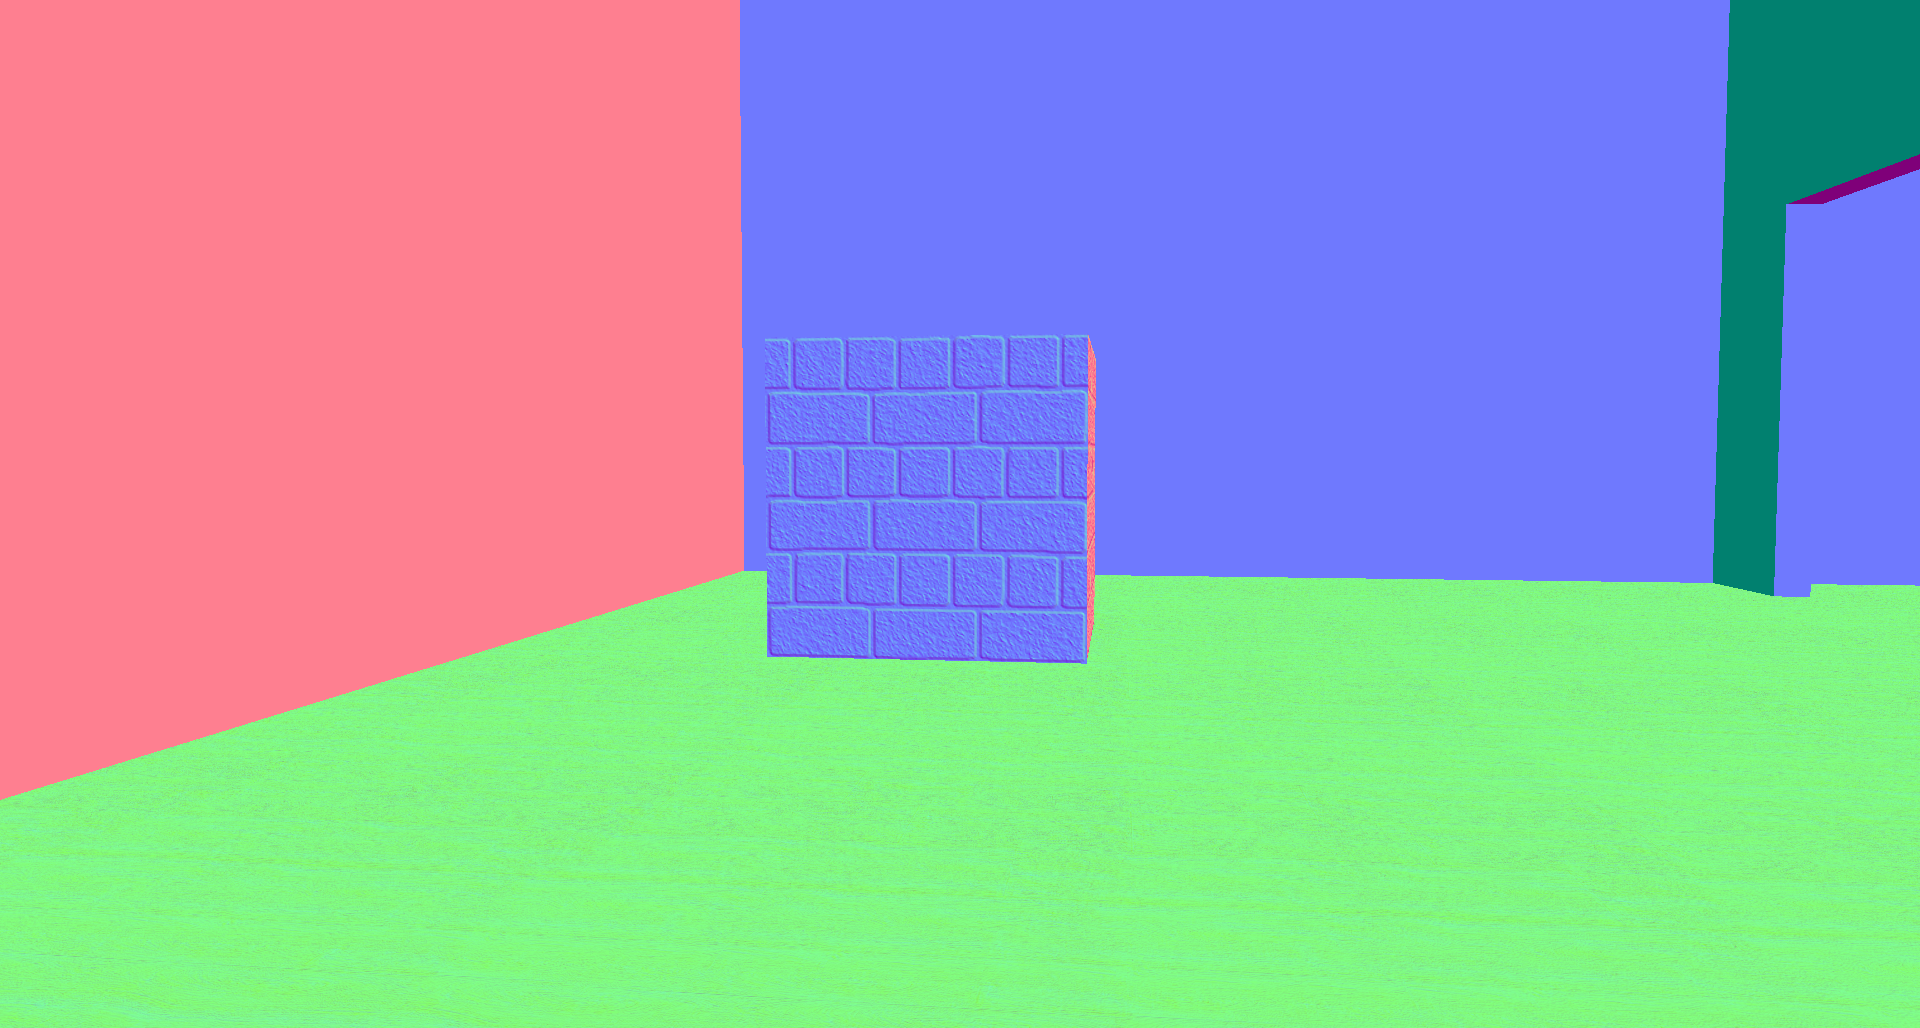
\includegraphics[width=1.0\textwidth]{normal_mapping_normal}
        \caption{Normal Texture with Brick Normal Mapping}
      \end{figure}

      \begin{figure}[h!]
        \centering
        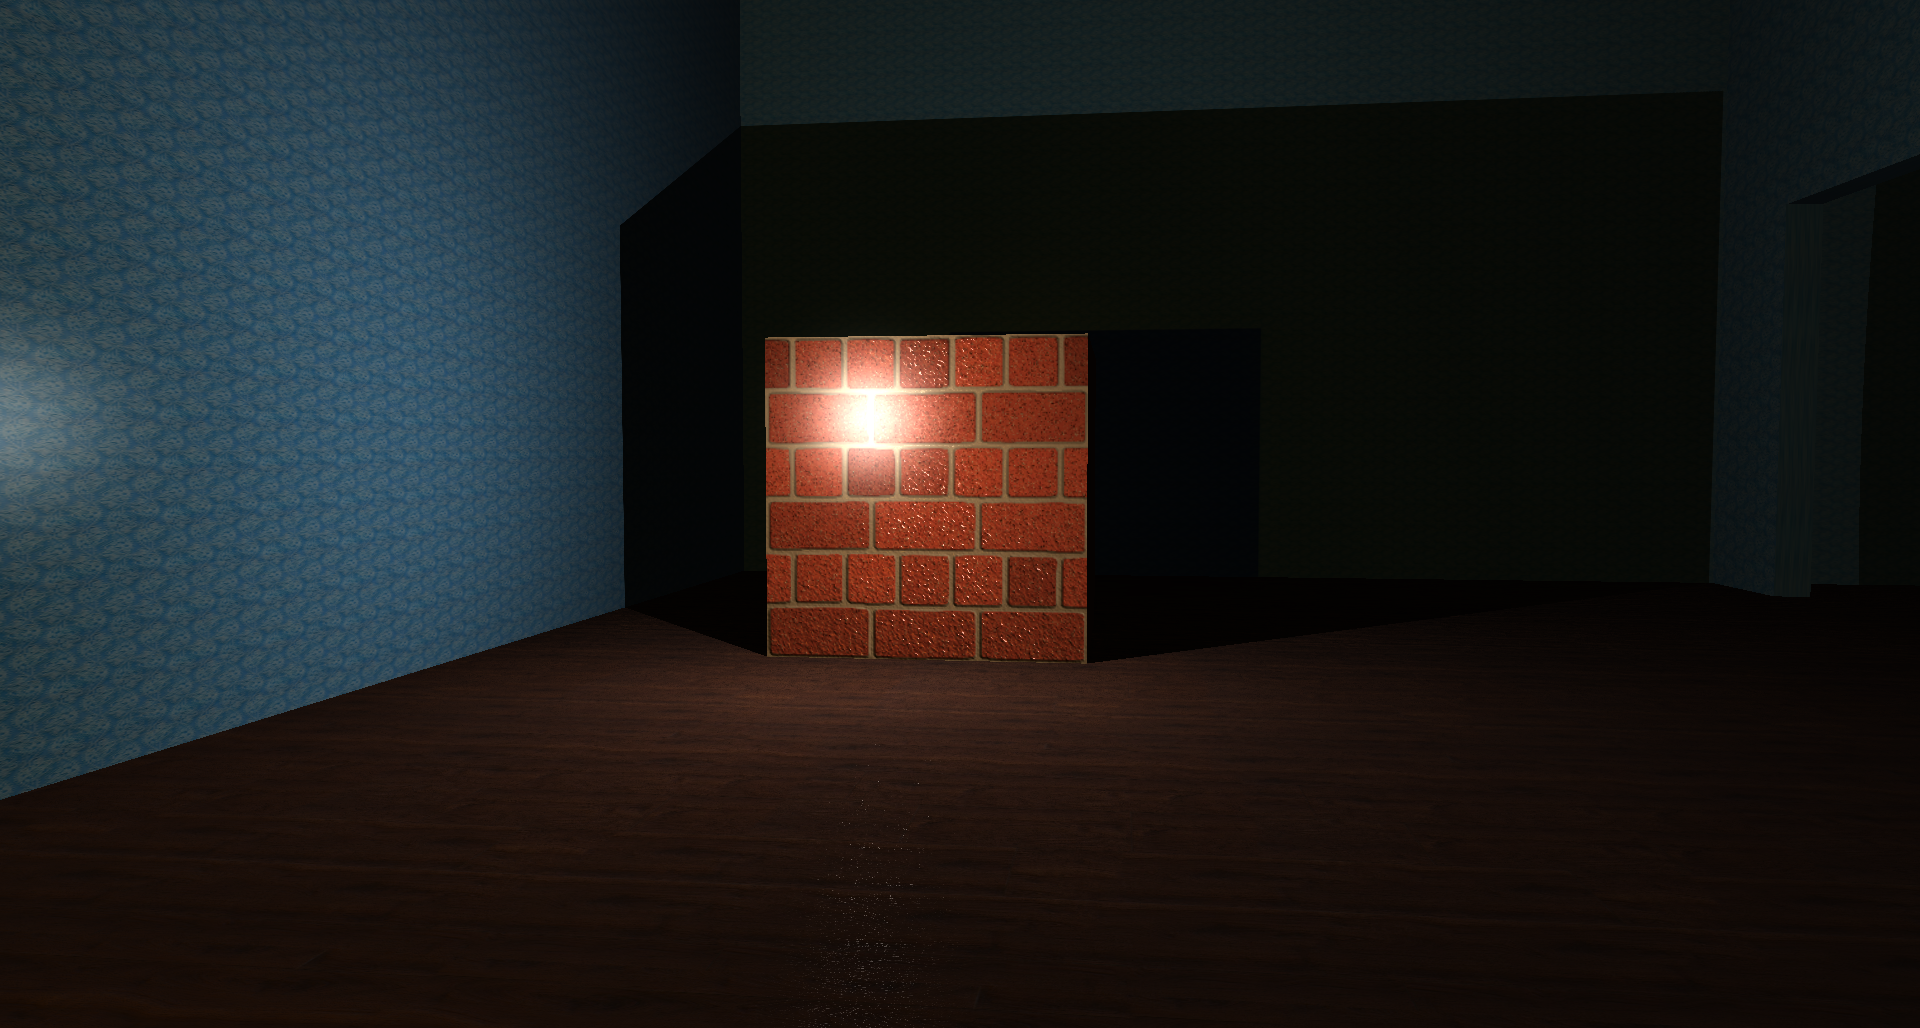
\includegraphics[width=1.0\textwidth]{normal_mapping_accum}
        \caption{Render with Brick Normal Mapping}
        \label{brick-normal-map}
      \end{figure}

      Normal mapping is when, usually in addition to a diffuse colour texture, you have a texture representing how normals should be perturbed at each pixel of the texture. The x, y, and z values of a normal are stored as the RGB values of the pixel. This technique lets you have very detailed bumps on a surface that would take millions of extra polygons to construct using only geometry. These normal vectors are stored in tangent space, and have to be converted to model space in order to be used for lighting calculations. I do this by pre-computing tangent and bitangent vectors on the CPU when loading models (see src/mesh.cpp:83-100). Then in the Geometry Pass Shader I compute a tangent-bitangent-normal matrix (TBN) to convert these to model space (see shaders/geomTextures.frag:64-71). These normals are then used to perform the regular shading calculations in the Deferred Rendering Shader (see shaders/deferredShading.frag:146).

      I followed a helpful tutorial at http://www.opengl-tutorial.org/intermediate-tutorials/tutorial-13-normal-mapping/.

    \subsection{Shadow Mapping} \label{shadow-mapping}
      The regular shadow mapping algorithm is well-known and consists of a first pass where geometry is rendered from the perspective of a dynamic light source, and only a depth buffer is written \cite{williams1978casting}. This is done for each light. Then a second pass can perform lighting calculations based off of whether the camera's perspective sees pixels that are farther or closer than the first surface each light sees is.

      This algorithm is compatible with deferred-rendering and in fact allows you to use more dynamic light sources because they only have to perform shading for each fragment instead of for each vertex (see shaders/deferredShading.frag:235-291). See Figure \ref{brick-normal-map} for a screenshot of point light shadow mapping.

      Three light source types were be implemented (see src/light.hpp).
      \begin{enumerate}
        \item Directional Lights - no position or falloff and parallel light rays.
        \item Spot Lights - position, direction, angle, and falloff
        \item Point Lights - position and falloff, lights in all directions.
      \end{enumerate}

      Shadow mapping was the most challenging to implement for point lights because a texture cube map will need to be used, which is created by doing 6 normal shadow map passes in each of the directions of a cube at the light source. However, GLSL has a cube map texture sampler to make it easy to sample the correct face of the cube.

      There are multiple extensions to shadow mapping that eliminate visual artifacts present in the basic implementation and allow more realistic penumbrae, but they were outside the scope of this project \cite{dimitrov2007cascaded} \cite{fernando2005percentage}.

      I followed a helpful tutorial at http://www.opengl-tutorial.org/intermediate-tutorials/tutorial-16-shadow-mapping/.

    \subsection{SSAO} \label{ssao}
      \begin{figure}[h!]
        \centering
        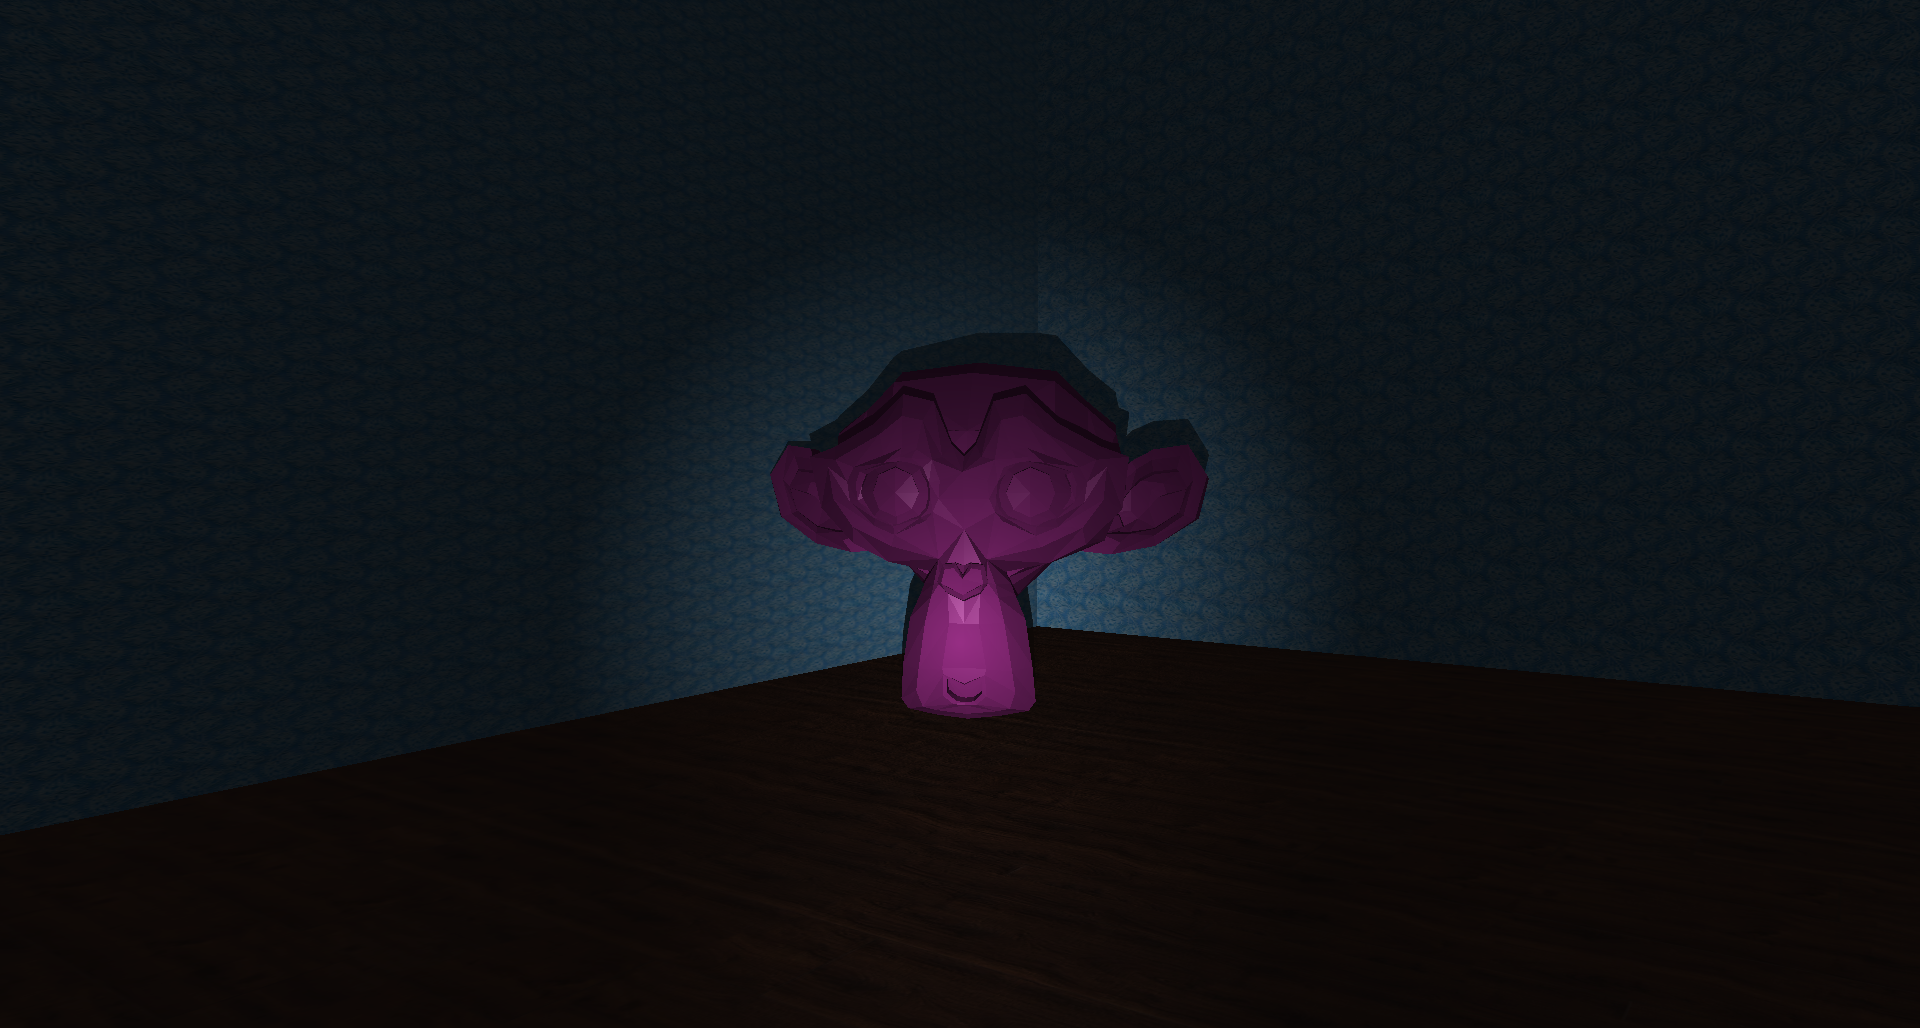
\includegraphics[width=1.0\textwidth]{nossao}
        \caption{SSAO turned off}
      \end{figure}

      \begin{figure}[h!]
        \centering
        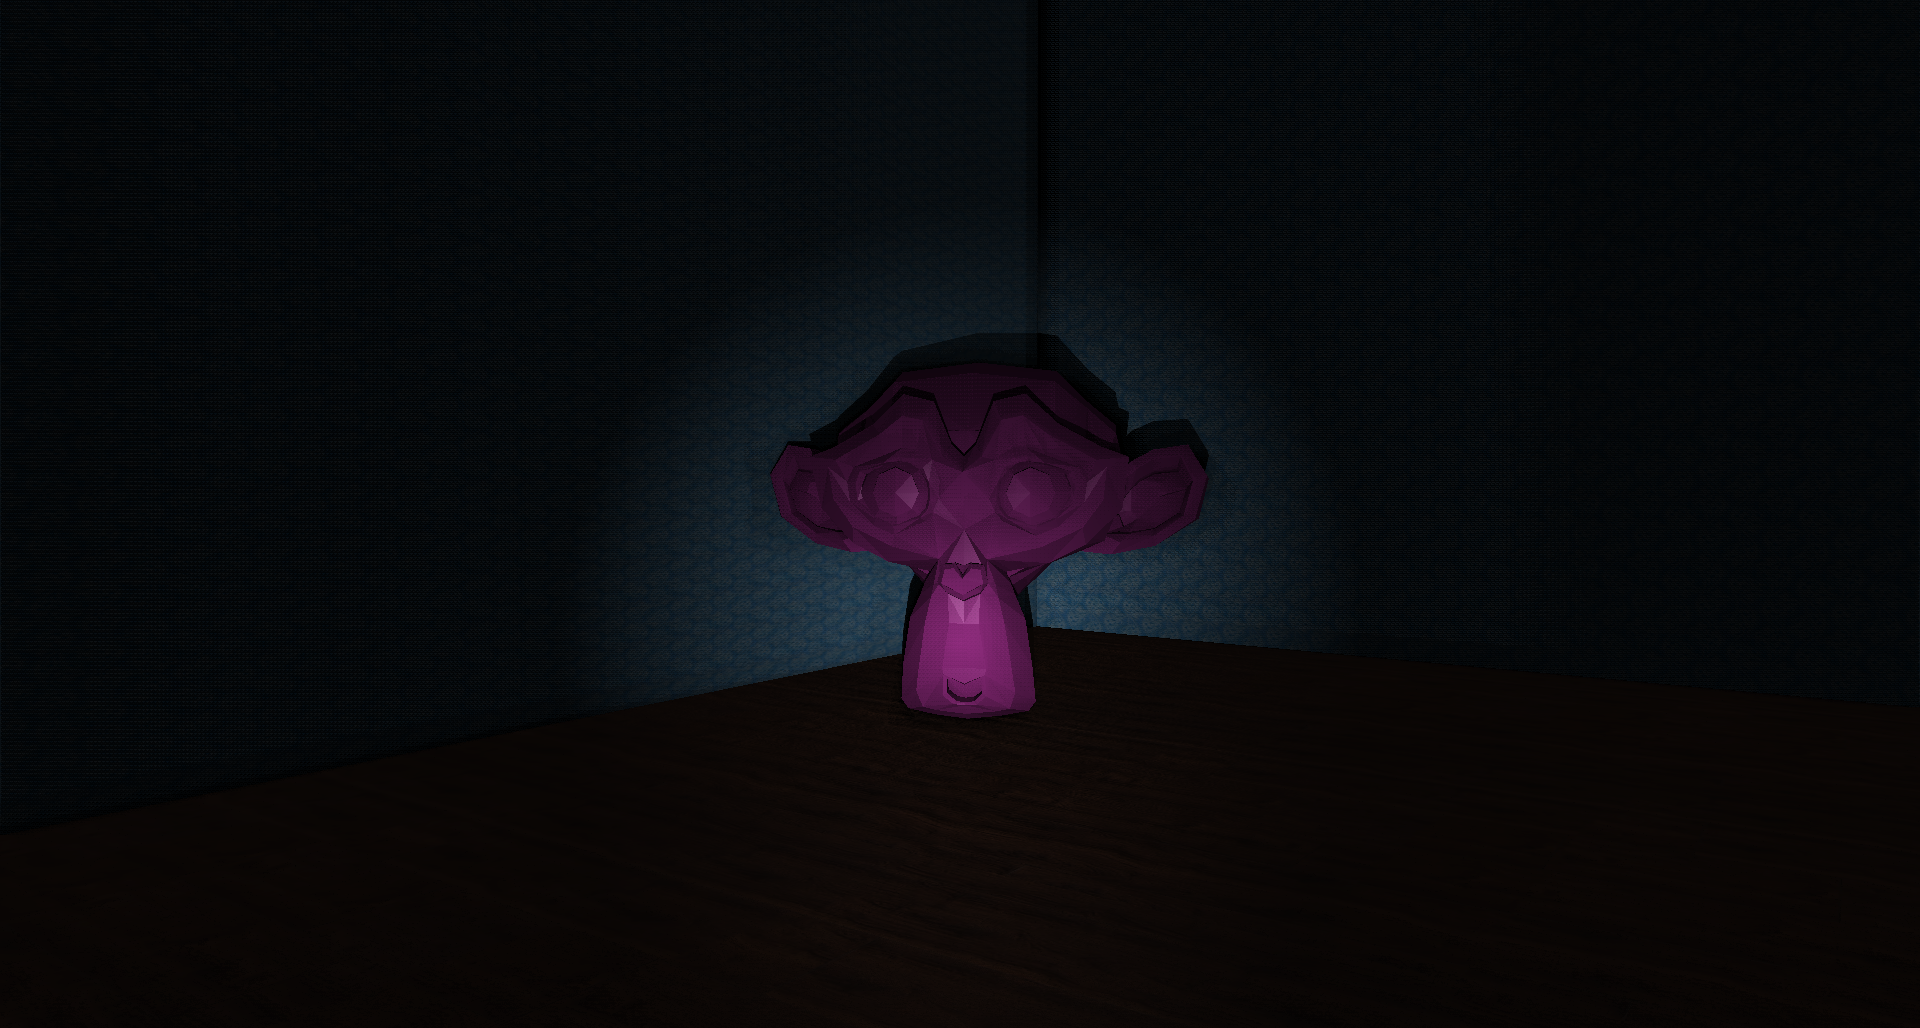
\includegraphics[width=1.0\textwidth]{ssao}
        \caption{SSAO turned on}
      \end{figure}

      Ambient Occlusion means calculating an occlusion factor that can be applied to the ambient light term to improve lighting correctness. There is more than one fast algorithm for this, but this project uses the quick algorithm named Screen Space Ambient Occlusion \cite{kajalinshaderx7}\cite{mittring2007finding}.

      The algorithm works by sampling the depth of neighbouring pixels to determine whether a fragment should receive more or less ambient light. From the depth and normal information of each fragment, a view-space position and normal can be computed. Sample positions within a hemisphere oriented along the fragment's normal are selected based off of a pre-computed kernel and rotated randomly based off of a noise texture. These sample points are projected onto screenspace and the depth texture is sampled to see whether these points are in front of the fragment being shaded. The fraction of sampled points that are in front of the fragment being shaded is used to decrease the ambient shading factor for this fragment. See shaders/deferredShading.frag:304-315,68-89.

      I followed a helpful tutorial at http://john-chapman-graphics.blogspot.ca/2013/01/ssao-tutorial.html?m=1.


    \subsection{Motion Blur} \label{motion-blur}
      Motion blur is a an effect that blurs objects when move your camera. The amount of blur is proportinal to the speed of movement of the vectors/pixels on the screen.
      I implemented a screen-space technique that runs in the post-processing shader. The technique is based off of this tutorial: http://john-chapman-graphics.blogspot.ca/2013/01/what-is-motion-blur-motion-pictures-are.html.

      The algorithm is to approximate where each pixel would have been in the last frame by storing the previous frame's view matrix, and blurring by sampling along the delta vector for each fragment. A matrix is computed and passed to the shader that maps the current frame's screenspace coordinates to the previous frame's screenspace coordinates. With this matrix a blur vector is computed by subtracting the two screenspace positions. Fragments are sampled along this blur vector and blended together to get the blurring effect. See shaders/postProcess.frag:69-86.

      This technique is affected by frame rate, since if the frame rate is very high, then the previous view matrix will be almost the same and almost no blurring will occur. This can be fixed by calculating the frame rate and passing the shader a correction factor.


    \subsection{Planar Mirrors} \label{mirrors}
      Planar mirror reflections are implemented by rendering the complete scene an extra time to texture, and then applying the texture to a quad when rendering from the camera's perspective. Each frame, before starting the rendering pipeline, the rendering pipeline is invoked for each mirror and rendered to a texture (see src/viewer.cpp:1068-1093 and src/mirror.cpp:58). For this invocation, instead of the camera's view, a reflection of the camera's viewing frustum about the mirror is used. The target texture is owned by the mirror, and it uses it as a source texture for subsequent renders. An important step is to set the UV coordinates of the quad that represents the mirror to the geometry of the quad projected in the reflected viewing frustum's perspective. I came up with this technique on my own (with some inspiration from posts on the internet). See Figure \ref{screenshot01} for a screenshot.


    \subsection{Shader Picking} \label{picking}
      I use a simple picking technique that leverages the fact that a fragment shader can be told the Id of the mesh it is rendering, and that Id can be stored in a texture. Then to pick I simply read the center pixel of the picking texture and recover the Id of the mesh the player is looking at. See src/viewer.cpp:695-700.



  \section{Implementation}
  %TODO
%Algorithms, data structures, and complexities,
%• Modularity, data abstraction and encapsulation,
%• Platform and system dependence or independence, global constants and configurability,
%• Data and code sources, network and literature resources, system and local utilities, the
%re-use and adaptation of existing code,
%delegation,
%• Coding style, debugging approach and utilities, version management, testing and veri-
%fying practices,
%• Caveats, bugs, cautions, unexplored areas, assumptions, future possibilities.


    %TODO - Acknowledgements.


    % References.

    %\begingroup
    %\renewcommand{\section}[2]{}%
    \nocite{*}
    \bibliography{biblio}{}
    \bibliographystyle{plain}
    %\endgroup
\newpage


%\chapter{Objectives}

%{\hfill{\bf Full UserID: ayklen}\hfill{\bf Student ID: 20372654}\hfill}

%\begin{enumerate}
  %\item[\_\_\_ 1:]  Modelled environment that shows off dynamic shadows with many light sources.

  %\item[\_\_\_ 2:]  Interactive first-person controls and interaction with environment (UI).

  %\item[\_\_\_ 3:]  Real-time Shadow Maps in shader for dynamic shadows. Standard implementation with comparisons against depth textures generated from the perspective of each light.

  %\item[\_\_\_ 4:]  Texture Mapping in shader.

  %\item[\_\_\_ 5:]  Bump/Normal Mapping in shader.

  %\item[\_\_\_ 6:]  Motion blur implemented as a post-processing shader pass.

  %\item[\_\_\_ 7:]  Ambient Occlusion approximation in shader using Screen Space Ambient Occlusion (SSAO). Decreases ambient light contribution for pixels that are occluded by sampled neighboring pixels (using depths and normals in screen space).

  %\item[\_\_\_ 8:]  Sound synchronized with game.

  %\item[\_\_\_ 9:]  Planar mirror reflection. Find reflected ray off of mirror surface, render scene to texture from ray's perspective, render scene from camera's perspective while applying texture to mirror geometry.

  %\item[\_\_\_ 10:] Keyframe Animation.
%\end{enumerate}

\end{document}
